\documentclass[11pt, a4paper]{article}

\usepackage[a4paper, margin=2.3cm]{geometry}
\usepackage[utf8]{inputenc}
\usepackage[T1]{fontenc}
\usepackage{lmodern}
\usepackage[english]{babel}

\usepackage{amsmath, amssymb, amsthm}
\usepackage{booktabs}
\usepackage{enumitem}
\usepackage{xcolor}
\usepackage{tikz}
\usetikzlibrary{arrows.meta, positioning, calc, shapes.geometric, patterns}
\usepackage{hyperref}

% Color Palette
\definecolor{primaryblue}{RGB}{24, 90, 169}
\definecolor{lightbg}{RGB}{240, 246, 255}
\definecolor{formalbg}{RGB}{248, 249, 250}
\definecolor{formalborder}{RGB}{100, 116, 139}
\definecolor{accentorange}{RGB}{217, 119, 6}
\definecolor{accentgreen}{RGB}{22, 163, 74}
\definecolor{accentpurple}{RGB}{126, 34, 206}
\definecolor{amber}{RGB}{245, 158, 11}
\definecolor{emerald}{RGB}{16, 185, 129}

\hypersetup{
    colorlinks=true,
    linkcolor=primaryblue,
    urlcolor=primaryblue,
    citecolor=primaryblue
}

% Theorem Environments
\theoremstyle{definition}
\newtheorem{definition}{Definition}[section]
\newtheorem{theorem}[definition]{Theorem}
\newtheorem{proposition}[definition]{Proposition}
\newtheorem{lemma}[definition]{Lemma}
\newtheorem{corollary}[definition]{Corollary}
\newtheorem{example}[definition]{Example}
\newtheorem{algorithm_env}[definition]{Algorithm}

% Safe Boxed Environments (No external tcolorbox dependency required)
\newcommand{\intuitionbox}[2]{%
    \par\medskip\noindent
    \fcolorbox{primaryblue}{lightbg}{%
        \parbox{\dimexpr\linewidth-2\fboxsep-2\fboxrule\relax}{%
            \vspace{2pt}
            \textcolor{primaryblue}{\textbf{Intuition — #1}}\par\smallskip
            #2
            \vspace{2pt}
        }%
    }\par\medskip
}

\newcommand{\formalbox}[1]{%
    \par\medskip\noindent
    \fcolorbox{formalborder}{formalbg}{%
        \parbox{\dimexpr\linewidth-2\fboxsep-2\fboxrule\relax}{%
            \vspace{2pt}
            #1
            \vspace{2pt}
        }%
    }\par\medskip
}

\newcommand{\imageplaceholder}[3]{%
    \par\medskip\noindent
    \begin{center}
    \fcolorbox{formalborder}{white}{%
        \parbox{0.92\linewidth}{%
            \vspace{14pt}
            \centering
            \textbf{\textcolor{formalborder}{[ IMAGE PLACEHOLDER — Insert from #1 ]}}\\[6pt]
            \small\textit{Visual Description:} #2\\[8pt]
            \footnotesize\textbf{Suggested Caption:} #3
            \vspace{14pt}
        }%
    }
    \end{center}
    \par\medskip
}

\title{\textbf{Foundations of Spatial AI}\\[4pt]
\Large Lecture 12: Gaussian-Based Active Planning}
\author{Based on lectures by \textbf{Valerio Spagnoli}\\
Sapienza University of Rome (\texttt{rvp-group.github.io/sai-teaching})}
\date{November 2, 2026}

\begin{document}

\maketitle

\begin{abstract}
\noindent These lecture notes provide a rigorous and self-contained mathematical and algorithmic treatment of \textbf{Lecture 12: Gaussian-Based Active Planning} from the \emph{Foundations of Spatial AI (2026/27)} course. We trace the transition from passive scene reconstruction to active perception and Next-Best-Pose planning, examine how \textbf{3D Gaussian Splatting (3DGS)} acts as a fast differentiable rendering engine for scoring candidate camera trajectories, analyze coverage-driven planning with \textbf{MAGICIAN}, and study a complete online semantic object-mapping architecture combining a 5\,cm voxel planning state with multi-channel Gaussian signal rendering and horizon-5 beam search.
\end{abstract}

\tableofcontents
\newpage

% ============================================================================
\section{Active Perception and Active Mapping \emph{(slides 1--4)}}
% ============================================================================

\subsection{What Is Active Perception? \emph{(slides 1--2)}}

Classical computer vision and spatial mapping pipelines often operate in a \textbf{passive} regime: a fixed sequence of sensor measurements is handed to the algorithm, which processes whatever arrives. In robotics and embodied AI, however, an agent controls its own motion and camera pose. This leads to the paradigm of \textbf{Active Perception}:
\begin{quote}
\emph{``What we perceive depends on what we decide to do.''}
\end{quote}

\formalbox{
\begin{definition}[Passive vs.\ Active Perception]
Let $\mathcal{X}$ denote the space of sensor observations (e.g., RGB-D frames), $\mathcal{T} \subset \mathrm{SE}(3)$ the space of feasible camera poses, and $\mathcal{M}$ the space of internal scene representations (maps).
\begin{itemize}[leftmargin=*]
    \item \textbf{Passive Perception:} Given an exogenous sequence of observations $\{(I_t, D_t, T_t)\}_{t=1}^N$, the estimation algorithm computes a map $M_N = \Phi(\{(I_t, D_t, T_t)\}_{t=1}^N)$ without influencing the poses $T_t$.
    \item \textbf{Active Perception:} At each discrete step $t$, the agent maintains a map $M_t \in \mathcal{M}$ updated from past observations and applies a decision policy $\pi: \mathcal{M} \times \mathcal{T}_{\text{task}} \to \mathcal{T}$ that selects the next viewpoint $T_{t+1} = \pi(M_t, \tau)$ conditioned on the task $\tau$, physically moves to $T_{t+1}$, and acquires $(I_{t+1}, D_{t+1})$.
\end{itemize}
\end{definition}
}

\begin{figure}[htbp]
\centering
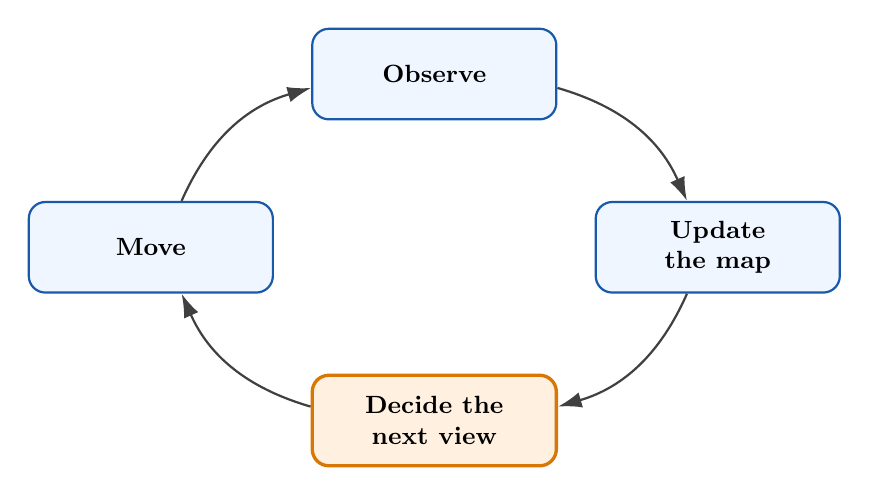
\begin{tikzpicture}[
    node distance=2.2cm and 3.2cm,
    box/.style={rectangle, rounded corners=6pt, draw=primaryblue, thick, fill=lightbg, minimum width=3.1cm, minimum height=1.15cm, align=center, font=\small\bfseries},
    decidebox/.style={rectangle, rounded corners=6pt, draw=accentorange, very thick, fill=orange!12, minimum width=3.1cm, minimum height=1.15cm, align=center, font=\small\bfseries},
    arrow/.style={-{Latex[length=3mm, width=2mm]}, thick, draw=darkgray}
]
    \node[box] (obs) at (0, 2.2) {Observe};
    \node[box] (upd) at (3.6, 0) {Update\\the map};
    \node[decidebox] (dec) at (0, -2.2) {Decide the\\next view};
    \node[box] (mov) at (-3.6, 0) {Move};

    \draw[arrow] (obs) to[bend left=25] (upd);
    \draw[arrow] (upd) to[bend left=25] (dec);
    \draw[arrow] (dec) to[bend left=25] (mov);
    \draw[arrow] (mov) to[bend left=25] (obs);
\end{tikzpicture}
\caption{The closed-loop Active Perception cycle (redrawn from Slide 2). The highlighted orange block (\emph{Decide the next view}) closes the loop between mapping and physical camera motion.}
\label{fig:active_loop}
\end{figure}

\intuitionbox{Why Passive Data Collection Fails Under a Budget}{
Imagine walking into a cluttered living room with a camera and only being allowed to take $N=50$ photographs. A passive agent moving along a pre-programmed path might spend 30 frames staring at a blank white wall or the floor, leaving complex furniture occluded or blurry. An active agent inspects its current partial map after every frame and asks: \emph{``Where is my map still incomplete or uncertain, and which camera movement will fix that fastest?''}
}

\subsection{Active Mapping \emph{(slide 3)}}

When the specific task $\tau$ is to reconstruct a complete 3D scene within a strict budget of views $B$, active perception specializes to \textbf{Active Mapping} (also known as the \textbf{Next-Best-View} or \textbf{Next-Best-Pose} problem).

At each discrete time step $t \in \{1, 2, \dots, B\}$, the system receives an input tuple consisting of:
\begin{enumerate}[leftmargin=*]
    \item \textbf{Color frame} $I_t \in \mathbb{R}^{H \times W \times 3}$ (RGB image),
    \item \textbf{Depth frame} $D_t \in \mathbb{R}_+^{H \times W}$ (metric depth per pixel),
    \item \textbf{Camera pose} $T_t \in \mathrm{SE}(3)$ (the 6-DoF position and orientation in world coordinates).
\end{enumerate}

\begin{figure}[htbp]
\centering
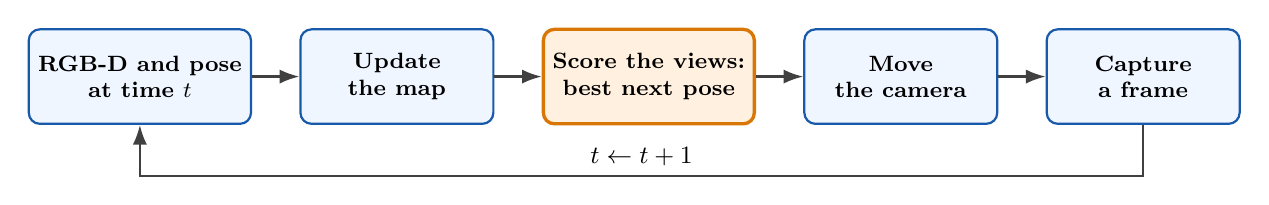
\begin{tikzpicture}[
    node distance=0.6cm,
    pbox/.style={rectangle, rounded corners=4pt, draw=primaryblue, thick, fill=lightbg, minimum width=2.45cm, minimum height=1.2cm, align=center, font=\footnotesize\bfseries},
    scorebox/.style={rectangle, rounded corners=4pt, draw=accentorange, very thick, fill=orange!12, minimum width=2.65cm, minimum height=1.2cm, align=center, font=\footnotesize\bfseries},
    arr/.style={-{Latex[length=2.5mm, width=1.8mm]}, thick, draw=darkgray}
]
    \node[pbox] (n1) {RGB-D and pose\\at time $t$};
    \node[pbox, right=of n1] (n2) {Update\\the map};
    \node[scorebox, right=of n2] (n3) {Score the views:\\best next pose};
    \node[pbox, right=of n3] (n4) {Move\\the camera};
    \node[pbox, right=of n4] (n5) {Capture\\a frame};

    \draw[arr] (n1) -- (n2);
    \draw[arr] (n2) -- (n3);
    \draw[arr] (n3) -- (n4);
    \draw[arr] (n4) -- (n5);

    \draw[arr] (n5.south) -- ++(0,-0.65) -- node[above, font=\small\bfseries] {$t \leftarrow t + 1$} ($(n1.south)+(0,-0.65)$) -- (n1.south);
\end{tikzpicture}
\caption{The sequential Active Mapping loop (redrawn from Slide 3). At each step $t$, the map is updated with $(I_t, D_t, T_t)$, candidate viewpoints are scored, and the camera moves to capture frame $t+1$.}
\label{fig:active_mapping_pipeline}
\end{figure}

\imageplaceholder{Slide 3 (top right)}{Photorealistic 3D reconstruction of an indoor living room scene (white sofas, wooden coffee table, armchairs, floor lamp, window blinds) alongside stacked historical input frames (Color, Depth, Pose $T_t$).}{Figure: Input stream of RGB, Depth, and camera poses $T_t$ (left) and the online reconstructed 3D scene map (right) from Slide 3.}

\subsection{Our Task: Focus on the Objects \emph{(slide 4)}}

Standard active mapping treats every square meter of surface area identically: a bare wall or carpet tile receives the same priority as an intricate object on a table. Slide 4 introduces the core thesis of this lecture:
\begin{quote}
\emph{``Not all surfaces matter the same: we care about the objects of the scene. To focus on objects, the robot must know what they are: we need semantics.''}
\end{quote}

\formalbox{
\begin{definition}[Semantic Object-Centric Active Mapping]
Let $\mathcal{C} = \{1, \dots, K\}$ be a set of semantic categories split into \textbf{background/structural classes} $\mathcal{C}_{\text{bg}}$ (e.g., wall, floor, ceiling) and \textbf{foreground object classes} $\mathcal{C}_{\text{obj}}$ (e.g., chair, cushion, vase, table, lamp). Given a view budget $B$, the objective of \textbf{Semantic Object-Centric Active Mapping} is to select a trajectory of poses $\tau = (T_1, \dots, T_B) \in \mathcal{T}^B$ that maximizes the geometric completeness, spatial resolution (proximity), multi-angle coverage, and semantic classification accuracy across all object instances $o \in \mathcal{O}$ belonging to $\mathcal{C}_{\text{obj}}$.
\end{definition}
}

To achieve this, the pipeline augments the raw RGB-D input with a 2D semantic segmenter (such as \textbf{OneFormer}) that predicts pixel-wise class labels, fuses those labels into the 3D representation, and directs the planner toward object regions requiring closer or novel viewing angles.

\imageplaceholder{Slide 4}{Four-panel visual summary showing: (1) Input: split RGB and depth image; (2) Classes from a segmenter (color-coded semantic segmentation mask); (3) Where the robot should look (3D grey mesh with bright orange highlighted target objects like pillows, coffee table items, side tables); (4) The map: split view showing photorealistic RGB and semantic class colors.}{Figure: Overview of object-centric semantic active mapping (Slide 4), highlighting how semantic segmentation guides the planner to focus on scene objects (orange) rather than structural background.}

% ============================================================================
\section{The Tool: 3D Gaussian Splatting \emph{(slides 5--8)}}
% ============================================================================

\subsection{3D Gaussian Splatting Representation \emph{(slide 5)}}

To both represent the scene at high visual fidelity and rapidly evaluate candidate viewpoints, the system builds upon \textbf{3D Gaussian Splatting (3DGS)} (Kerbl et al., ACM TOG 2023). Rather than using an implicit neural radiance field (NeRF) that requires costly volumetric ray-marching through a multilayer perceptron (MLP), 3DGS represents a scene explicitly as a collection of $M$ anisotropic 3D Gaussians (often on the order of $1.0\text{ million}$ Gaussians for a room mapped from 50 views).

\formalbox{
\begin{definition}[Parameterized 3D Gaussian Primitive]
A 3D Gaussian primitive $g_k$ ($k \in \{1, \dots, M\}$) is defined by the parameter tuple
\[
g_k = \bigl(\boldsymbol{\mu}_k,\; \boldsymbol{\Sigma}_k,\; \alpha_k,\; \mathbf{c}_k,\; \mathbf{s}_k\bigr),
\]
where:
\begin{itemize}[leftmargin=*]
    \item \textbf{Position (Mean):} $\boldsymbol{\mu}_k \in \mathbb{R}^3$ is the 3D center in world coordinates.
    \item \textbf{Shape (Covariance):} $\boldsymbol{\Sigma}_k \in \mathbb{S}_{++}^3$ is a $3\times 3$ positive-definite covariance matrix defining the 3D ellipsoid's orientation and scale, parameterized via a rotation matrix $\mathbf{R}_k \in \mathrm{SO}(3)$ (stored as a unit quaternion) and a diagonal scaling matrix $\mathbf{S}_k = \mathrm{diag}(s_{k,x}, s_{k,y}, s_{k,z})$:
    \[
    \boldsymbol{\Sigma}_k = \mathbf{R}_k \mathbf{S}_k \mathbf{S}_k^\top \mathbf{R}_k^\top.
    \]
    \item \textbf{Opacity:} $\alpha_k \in [0, 1]$ controls the radiative absorption/blending weight of the primitive.
    \item \textbf{Color:} $\mathbf{c}_k \in [0, 1]^3$ (or spherical harmonics coefficients) represents the RGB appearance.
    \item \textbf{Semantic / Utility Payload:} $\mathbf{s}_k$ stores task-specific attributes, such as semantic class vote slots or planning signal values.
\end{itemize}
The unnormalized 3D spatial density of Gaussian $k$ at point $\mathbf{x} \in \mathbb{R}^3$ is:
\[
G_k(\mathbf{x}) = \exp\left( -\frac{1}{2} (\mathbf{x} - \boldsymbol{\mu}_k)^\top \boldsymbol{\Sigma}_k^{-1} (\mathbf{x} - \boldsymbol{\mu}_k) \right).
\]
\end{definition}
}

\imageplaceholder{Slide 5}{Three-part figure of a reconstructed room from 50 views using 1.0 million Gaussians: (left) full 3D view of the room showing sofa, chairs, and table; (top right) close-up RGB render ('Color - 50 views'); (bottom right) close-up semantic render ('Classes - 50 views').}{Figure: A living room represented by 1.0 million 3D Gaussians trained from 50 views, rendering both photorealistic color and dense semantic classes (Slide 5).}

\subsection{How Does 3DGS Work? \emph{(slide 6)}}

To render an image from a camera pose $T = (\mathbf{R}_c, \mathbf{t}_c) \in \mathrm{SE}(3)$, 3DGS projects each 3D Gaussian into the 2D image plane, sorts the Gaussians intersecting each pixel ray from front to back by depth, and alpha-composits their colors.

\formalbox{
\begin{proposition}[Differentiable Splatting and Alpha-Compositing]
Given a viewing transformation $\mathbf{W}$ and the Jacobian $\mathbf{J}$ of the projective transformation at $\boldsymbol{\mu}_k$, the 3D covariance $\boldsymbol{\Sigma}_k$ projects to a 2D covariance matrix in pixel coordinates:
\[
\boldsymbol{\Sigma}'_k = \mathbf{J} \mathbf{W} \boldsymbol{\Sigma}_k \mathbf{W}^\top \mathbf{J}^\top.
\]
For a pixel $u \in \Omega$, let $\{1, \dots, K_u\}$ index the Gaussians overlapping $u$ sorted in ascending order of camera depth $z_1 \le z_2 \le \dots \le z_{K_u}$. The effective 2D opacity at pixel $u$ is $\tilde{\alpha}_k(u) = \alpha_k G'_k(u)$, where $G'_k(u)$ is the 2D Gaussian evaluated at $u$. The rendered color $\hat{\mathbf{c}}(u)$ is given by linear blending:
\begin{equation}
\hat{\mathbf{c}}(u) = \sum_{k=1}^{K_u} w_k(u)\, \mathbf{c}_k, \qquad \text{where} \qquad w_k(u) = \tilde{\alpha}_k(u) \prod_{j=1}^{k-1} \bigl(1 - \tilde{\alpha}_j(u)\bigr).
\label{eq:3dgs_render}
\end{equation}
Here $T_k(u) = \prod_{j=1}^{k-1} (1 - \tilde{\alpha}_j(u))$ is the accumulated transmittance from the camera to Gaussian $k$. During online training, the Gaussian parameters are optimized via gradient descent to minimize the pixel-wise photometric $\ell_1$ loss against the sensor image $\mathbf{c}(u)$:
\begin{equation}
\mathcal{L} = \sum_{u \in \Omega} \bigl| \hat{\mathbf{c}}(u) - \mathbf{c}(u) \bigr|.
\label{eq:3dgs_loss}
\end{equation}
\end{proposition}
}

\begin{figure}[htbp]
\centering
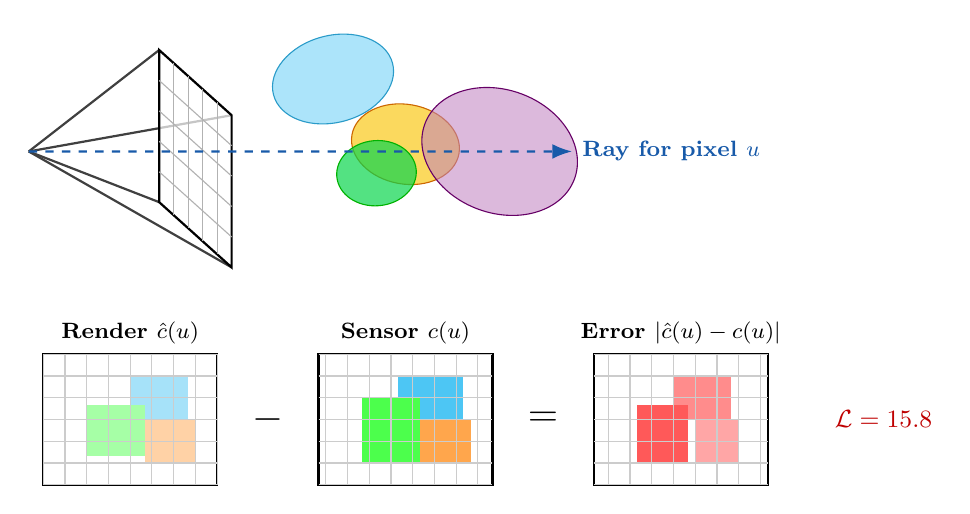
\begin{tikzpicture}[scale=0.92]
    % Camera Frustum
    \coordinate (cam) at (0, 1.8);
    \coordinate (p1) at (1.8, 3.2);
    \coordinate (p2) at (2.8, 2.3);
    \coordinate (p3) at (2.8, 0.2);
    \coordinate (p4) at (1.8, 1.1);

    \draw[thick, darkgray] (cam) -- (p1);
    \draw[thick, darkgray] (cam) -- (p2);
    \draw[thick, darkgray] (cam) -- (p3);
    \draw[thick, darkgray] (cam) -- (p4);
    \draw[thick, fill=white, fill opacity=0.7] (p1) -- (p2) -- (p3) -- (p4) -- cycle;

    % Grid on image plane
    \foreach \t in {0.2, 0.4, 0.6, 0.8} {
        \draw[thin, gray!60] ($(p1)!\t!(p4)$) -- ($(p2)!\t!(p3)$);
        \draw[thin, gray!60] ($(p1)!\t!(p2)$) -- ($(p4)!\t!(p3)$);
    }

    % 3D Gaussians (Ellipsoids)
    \filldraw[fill=cyan!50, draw=cyan!80!black, fill opacity=0.65, rotate around={15:(4.2,2.8)}] (4.2,2.8) ellipse (0.85cm and 0.6cm);
    \filldraw[fill=amber!60!yellow, draw=orange!80!black, fill opacity=0.65, rotate around={-10:(5.2,1.9)}] (5.2,1.9) ellipse (0.75cm and 0.55cm);
    \filldraw[fill=emerald!60!green, draw=green!70!black, fill opacity=0.7, rotate around={5:(4.8,1.5)}] (4.8,1.5) ellipse (0.55cm and 0.45cm);
    \filldraw[fill=violet!50, draw=violet!80!black, fill opacity=0.55, rotate around={-20:(6.5,1.8)}] (6.5,1.8) ellipse (1.1cm and 0.85cm);

    % Ray through pixel u
    \draw[-{Latex[length=2.5mm]}, thick, primaryblue, dashed] (cam) -- (7.5, 1.8) node[right, font=\footnotesize\bfseries] {Ray for pixel $u$};

    % Bottom pixel comparison panels
    \begin{scope}[yshift=-2.8cm, xshift=0.2cm]
        % Render grid
        \node[font=\footnotesize\bfseries] at (1.2, 2.1) {Render $\hat{c}(u)$};
        \draw[thick] (0,0) rectangle (2.4, 1.8);
        \fill[cyan!35] (1.2,0.9) rectangle (2.0,1.5);
        \fill[green!35] (0.6,0.4) rectangle (1.4,1.1);
        \fill[orange!35] (1.4,0.3) rectangle (2.1,0.9);
        \draw[step=0.3cm, gray!40, thin] (0,0) grid (2.4, 1.8);

        \node[font=\Large\bfseries] at (3.1, 0.9) {$-$};

        % Sensor grid
        \node[font=\footnotesize\bfseries] at (5.0, 2.1) {Sensor $c(u)$};
        \draw[thick] (3.8,0) rectangle (6.2, 1.8);
        \fill[cyan!70] (4.9,0.9) rectangle (5.8,1.5);
        \fill[green!70] (4.4,0.3) rectangle (5.2,1.2);
        \fill[orange!70] (5.2,0.3) rectangle (5.9,0.9);
        \draw[step=0.3cm, gray!40, thin] (3.8,0) grid (6.2, 1.8);

        \node[font=\Large\bfseries] at (6.9, 0.9) {$=$};

        % Error grid
        \node[font=\footnotesize\bfseries] at (8.8, 2.1) {Error $|\hat{c}(u)-c(u)|$};
        \draw[thick] (7.6,0) rectangle (10.0, 1.8);
        \fill[red!45] (8.7,0.9) rectangle (9.5,1.5);
        \fill[red!65] (8.2,0.3) rectangle (8.9,1.1);
        \fill[red!35] (9.0,0.3) rectangle (9.6,0.9);
        \draw[step=0.3cm, gray!40, thin] (7.6,0) grid (10.0, 1.8);

        \node[font=\small\bfseries, text=red!75!black] at (11.6, 0.9) {$\mathcal{L} = 15.8$};
    \end{scope}
\end{tikzpicture}
\caption{Illustration of 3D Gaussian Splatting (redrawn from Slide 6). Anisotropic 3D Gaussians project onto the sensor grid via $\hat{c}(u) = \sum_k w_k(u)c_k$. Comparing the rendered image against the ground-truth sensor image pixel-by-pixel yields the photometric error map $|\hat{c}-c|$ and scalar loss $\mathcal{L} = \sum_u |\hat{c}(u) - c(u)|$.}
\label{fig:3dgs_work}
\end{figure}

\subsection{Training Views, Novel Views, and What a Planner Does with 3DGS \emph{(slides 7--8)}}

Once optimized on training views collected along the robot's trajectory, 3DGS supports \textbf{novel view synthesis} from arbitrary test viewpoints $T \in \mathrm{SE}(3)$ at hundreds of frames per second. Crucially, the exact same alpha-compositing equation \eqref{eq:3dgs_render} can render any modality attached to the Gaussians:
\begin{itemize}[leftmargin=*]
    \item \textbf{Rendered RGB:} replacing $\mathbf{c}_k$ with RGB color $\mathbf{c}_k \in [0,1]^3$,
    \item \textbf{Rendered Depth:} replacing $\mathbf{c}_k$ with the camera-frame $z$-depth $d_k(T)$ of Gaussian $k$,
    \item \textbf{Rendered Semantic Classes:} replacing $\mathbf{c}_k$ with the class label or class probability vector of Gaussian $k$.
\end{itemize}

Slide 8 poses the central insight linking 3DGS to active planning:
\begin{quote}
\emph{``3DGS is used for novel view synthesis, and rendering a new view is very fast. We use the renders to score a view for a task: $g(T, \tau) \in \mathbb{R}$.''}
\end{quote}

\formalbox{
\begin{definition}[Render-Based View Scoring Function]
Let $s_k(\tau, T) \in \mathbb{R}_{\ge 0}$ denote a task-dependent scalar (or multi-channel vector) utility assigned to Gaussian $g_k$ under task $\tau$ when viewed from candidate pose $T \in \mathrm{SE}(3)$. The \textbf{Render-Based View Score} $g(T, \tau) \in \mathbb{R}$ is computed by rendering the utility signal across the image plane $\Omega$ and summing over all pixels:
\begin{equation}
g(T, \tau) = \sum_{u \in \Omega} \hat{s}(u; T, \tau) = \sum_{u \in \Omega} \sum_{k=1}^{K_u} w_k(u; T)\, s_k(\tau, T).
\label{eq:view_score}
\end{equation}
\end{definition}
}

\intuitionbox{Why Rendering Solves Visibility and Occlusion for Free}{
In traditional active mapping, scoring a candidate pose $T$ requires casting thousands of rays through a 3D voxel grid to check which surfaces are visible and which are occluded by walls or furniture in front of them. Because 3DGS already sorts Gaussians front-to-back and multiplies by the transmittance $T_k(u) = \prod_{j < k}(1 - \tilde{\alpha}_j(u))$, occluded Gaussians behind a solid wall automatically receive weight $w_k(u; T) \approx 0$! Thus, \textbf{replacing a Gaussian's color with a task utility turns the fast GPU rasterizer into an occlusion-aware information-gain calculator}.
}

% ============================================================================
\section{MAGICIAN: Planning with Imagined Gaussians \emph{(slides 9--11)}}
% ============================================================================

\subsection{MAGICIAN Architecture and Imagined Gaussians \emph{(slides 9--10)}}

Before introducing our semantic object-focused system, Slides 9--10 examine a recent state-of-the-art baseline for coverage-driven active mapping: \textbf{MAGICIAN} (\emph{Li, S., et al., ``MAGICIAN: Efficient long-term planning with imagined Gaussians for active mapping,'' CVPR 2026}).

A fundamental challenge in active mapping is that standard 3DGS only places Gaussians on surfaces that have \emph{already been observed}. If the planner only renders existing Gaussians, a completely unexplored region appears empty and generates zero gain. MAGICIAN addresses this via three components:
\begin{enumerate}[leftmargin=*]
    \item \textbf{Imagined Gaussians:} A 3D \textbf{Volume Occupancy Network} takes the current reconstructed point cloud and RGB-D observations at time $t$ and predicts occupancy probabilities even in unobserved regions, instantiating \emph{Imagined Gaussians} over predicted surfaces.
    \item \textbf{Gain as a Novelty Render (Slide 10):} Each Imagined Gaussian is assigned:
    \[
    \text{opacity } \alpha_k = \text{predicted occupancy} \in [0,1], \qquad \text{color } c_k = \text{novelty} \in \{0, 1\},
    \]
    where novelty is $1$ (visualized as bright red) if the surface has not yet been covered and $0$ (grey) once seen. Rendering this novelty channel from a candidate pose $T$ and summing the pixel intensities directly computes the expected new surface coverage.
    \item \textbf{Long-Term Planning via Beam Search:} Rather than greedily selecting only the immediate next view $T_{t+1}$, MAGICIAN evaluates multi-step candidate trajectories $\tau_1, \dots, \tau_{N_b}$ of length $H$ using \textbf{beam search} to maximize cumulative coverage gain $G(\tau)$.
\end{enumerate}

\begin{figure}[htbp]
\centering
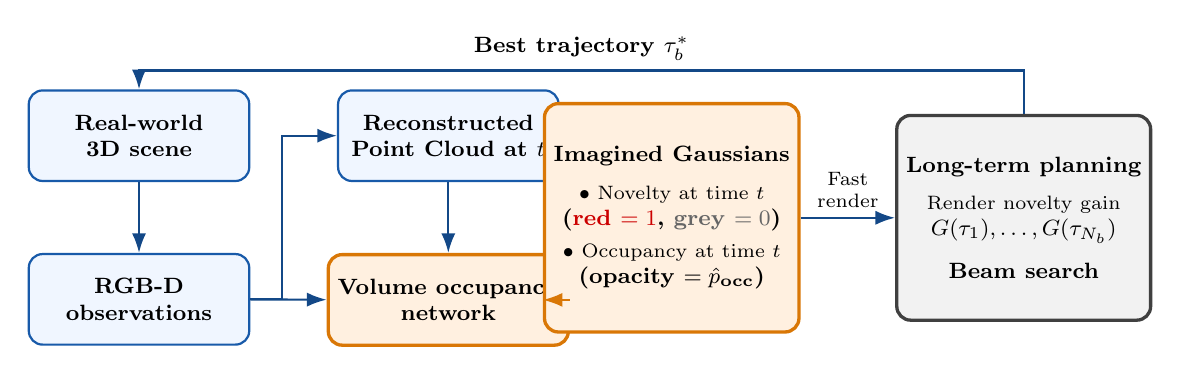
\begin{tikzpicture}[
    node distance=0.8cm and 1.1cm,
    block/.style={rectangle, rounded corners=5pt, draw=primaryblue, thick, fill=lightbg, minimum width=2.8cm, minimum height=1.15cm, align=center, font=\footnotesize\bfseries},
    netblock/.style={rectangle, rounded corners=5pt, draw=accentorange, very thick, fill=orange!12, minimum width=2.8cm, minimum height=1.15cm, align=center, font=\footnotesize\bfseries},
    planblock/.style={rectangle, rounded corners=5pt, draw=darkgray, very thick, fill=gray!10, minimum width=3.1cm, minimum height=2.6cm, align=center, font=\footnotesize\bfseries},
    arr/.style={-{Latex[length=2.5mm, width=1.8mm]}, thick, draw=primaryblue!80!black}
]
    \node[block] (scene) {Real-world\\3D scene};
    \node[block, below=0.9cm of scene] (rgbd) {RGB-D\\observations};
    \node[block, right=1.1cm of scene] (pcl) {Reconstructed\\Point Cloud at $t$};
    \node[netblock, below=0.9cm of pcl] (occnet) {Volume occupancy\\network};

    \node[netblock, right=1.2cm of $(pcl)!0.5!(occnet)$, minimum height=2.9cm, minimum width=3.2cm] (imag) {Imagined Gaussians\\[4pt]\normalfont\scriptsize $\bullet$ Novelty at time $t$\\(\textcolor{red!80!black}{red $=1$}, \textcolor{gray!80!black}{grey $=0$})\\[2pt]\normalfont\scriptsize $\bullet$ Occupancy at time $t$\\(opacity $= \hat{p}_{\text{occ}}$)};

    \node[planblock, right=1.2cm of imag] (beam) {Long-term planning\\[4pt]\normalfont\scriptsize Render novelty gain\\$G(\tau_1), \dots, G(\tau_{N_b})$\\[6pt]\textbf{Beam search}};

    \draw[arr] (scene) -- (rgbd);
    \draw[arr] (rgbd.east) -- ++(0.4,0) |- (pcl.west);
    \draw[arr] (rgbd) -- (occnet);
    \draw[arr] (pcl) -- (occnet);
    \draw[arr, draw=accentorange] (occnet.east) -- (imag.west |- occnet.east);
    \draw[arr] (imag) -- node[above, font=\scriptsize, align=center] {Fast\\render} (beam);
    \draw[arr] (beam.north) -- ++(0, 0.55) -| node[pos=0.25, above, font=\footnotesize\bfseries] {Best trajectory $\tau_b^*$} (scene.north);
\end{tikzpicture}
\caption{System architecture of MAGICIAN (redrawn from Slides 9--10). A volume occupancy network places Imagined Gaussians with opacity equal to predicted occupancy and color equal to novelty ($1=\text{unseen}$, $0=\text{seen}$), enabling rapid evaluation of multi-step trajectories via beam search.}
\label{fig:magician_arch}
\end{figure}

\imageplaceholder{Slide 10}{3D cutaway view of a room populated with regular spherical/ellipsoidal Gaussians colored bright red (novelty = 1, unseen surfaces on walls/furniture) and grey (novelty = 0, already observed floor/furniture surfaces).}{Figure: MAGICIAN's Imagined Gaussians in a room (Slide 10), where opacity encodes predicted occupancy and color encodes surface novelty (red = 1, grey = 0).}

\subsection{From Coverage to Objects \emph{(slide 11)}}

While MAGICIAN excels at rapid geometric exploration, Slide 11 highlights three critical limitations when the downstream robotics goal is object manipulation or semantic inspection:
\begin{enumerate}[leftmargin=*]
    \item \textbf{Single-glance saturation:} In pure coverage planning, once a surface is seen \emph{once}—even from $6\text{\,m}$ away at a grazing angle—its novelty drops to zero (\emph{``Once seen, a surface counts zero, however far away''}). Yet a distant, single-view observation produces distorted, incomplete 3D reconstructions with severe holes (as shown by the coffee-table vase comparison on Slide 11).
    \item \textbf{Lack of semantics:} \emph{``A book and a wall weigh the same: no semantics.''} Pure coverage wastes view budget mapping bare walls and floors at the same priority as tabletop objects.
    \item \textbf{Robotics motivation:} \emph{``Why: robots find, grasp and inspect objects; walls and floor are only where they move.''}
\end{enumerate}

\imageplaceholder{Slide 11 (top left)}{Side-by-side close-up comparison of a decorative vase on a wooden coffee table: 'Seen once to mark as covered' (severely torn, missing geometry, black holes) vs. 'Seen multiple times to map' (clean, complete, high-resolution cylindrical vase reconstruction).}{Figure: Seeing an object once from afar marks it as 'covered' in MAGICIAN but yields poor geometry (left), whereas seeing it from multiple close viewpoints yields an accurate 3D map (right) (Slide 11).}

% ============================================================================
\section{The Dual-Map System and Semantic Fusion \emph{(slides 12--17)}}
% ============================================================================

\subsection{The System and Full Pipeline \emph{(slides 12--13)}}

To map every object accurately along with its semantic class, our system maintains \textbf{two coupled representations} updated online from each posed RGB-D frame and OneFormer semantic segmentation mask:
\begin{enumerate}[leftmargin=*]
    \item \textbf{Online Gaussian Map (the final map):} Trained online from RGB-D frames and pixel classes; stores color, geometry, and semantic class votes. It serves both as the final high-resolution output map and as the fast differentiable renderer used by the planner.
    \item \textbf{Voxel Map (the planning state):} Built from depth measurements alone at $5\text{\,cm}$ resolution (with semantic class copied from the Gaussians inside each voxel). It tracks where the robot can safely fly (free vs.\ occupied vs.\ unknown space) and records detailed observation statistics per surface voxel: closest viewing distance, viewing directions, and frontier status.
\end{enumerate}

\begin{figure}[htbp]
\centering
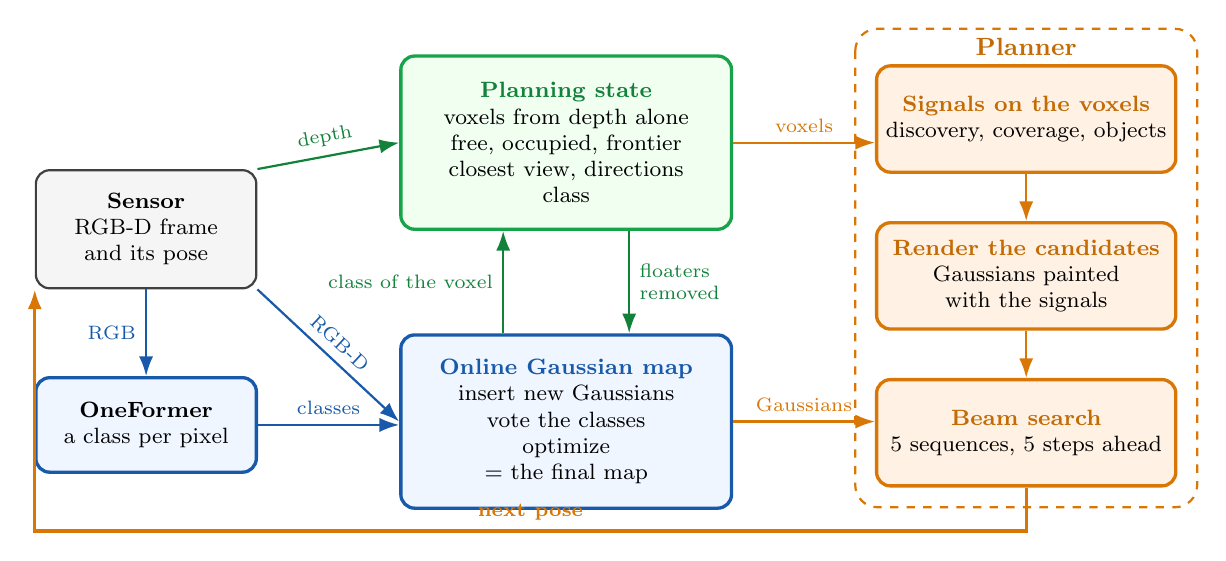
\begin{tikzpicture}[
    node distance=0.9cm and 1.4cm,
    sensorbox/.style={rectangle, rounded corners=5pt, draw=darkgray, thick, fill=gray!8, minimum width=2.8cm, minimum height=1.5cm, align=center, font=\footnotesize},
    segbox/.style={rectangle, rounded corners=5pt, draw=primaryblue, very thick, fill=lightbg, minimum width=2.8cm, minimum height=1.2cm, align=center, font=\footnotesize},
    gmap/.style={rectangle, rounded corners=5pt, draw=primaryblue, very thick, fill=lightbg, minimum width=4.2cm, minimum height=2.2cm, align=center, font=\footnotesize},
    vmap/.style={rectangle, rounded corners=5pt, draw=accentgreen, very thick, fill=green!6, minimum width=4.2cm, minimum height=2.2cm, align=center, font=\footnotesize},
    planbox/.style={rectangle, rounded corners=5pt, draw=accentorange, very thick, fill=orange!10, minimum width=3.8cm, minimum height=1.35cm, align=center, font=\footnotesize},
    arr/.style={-{Latex[length=2.5mm, width=1.8mm]}, thick}
]
    % Left column
    \node[sensorbox] (sensor) {\textbf{Sensor}\\RGB-D frame\\and its pose};
    \node[segbox, below=1.1cm of sensor] (oneformer) {\textbf{OneFormer}\\a class per pixel};

    % Middle column
    \node[vmap, right=1.8cm of sensor, yshift=1.1cm] (planningstate) {\textcolor{accentgreen!80!black}{\textbf{Planning state}}\\voxels from depth alone\\free, occupied, frontier\\closest view, directions\\class};
    \node[gmap, below=1.3cm of planningstate] (gaussianmap) {\textcolor{primaryblue}{\textbf{Online Gaussian map}}\\insert new Gaussians\\vote the classes\\optimize\\$=$ the final map};

    % Right column (Planner)
    \node[planbox, right=1.8cm of planningstate, yshift=0.3cm] (signals) {\textcolor{accentorange!90!black}{\textbf{Signals on the voxels}}\\discovery, coverage, objects};
    \node[planbox, below=0.6cm of signals] (render) {\textcolor{accentorange!90!black}{\textbf{Render the candidates}}\\Gaussians painted\\with the signals};
    \node[planbox, below=0.6cm of render] (beam) {\textcolor{accentorange!90!black}{\textbf{Beam search}}\\5 sequences, 5 steps ahead};

    % Dashed Planner Enclosure
    \draw[dashed, thick, accentorange, rounded corners=8pt]
        ($(signals.north west)+(-0.25,0.45)$) rectangle ($(beam.south east)+(0.25,-0.25)$);
    \node[font=\small\bfseries, text=accentorange!90!black] at ($(signals.north)+(0,0.22)$) {Planner};

    % Connections
    \draw[arr, accentgreen!80!black] (sensor.north east) -- node[above, sloped, font=\scriptsize] {depth} (planningstate.west);
    \draw[arr, primaryblue] (sensor.south east) -- node[above, sloped, font=\scriptsize] {RGB-D} (gaussianmap.west);
    \draw[arr, primaryblue] (sensor.south) -- node[left, font=\scriptsize] {RGB} (oneformer.north);
    \draw[arr, primaryblue] (oneformer.east) -- node[above, font=\scriptsize] {classes} (gaussianmap.west |- oneformer.east);

    % Bidirectional coupling between Voxel Map and Gaussian Map
    \draw[arr, accentgreen!80!black] ($(gaussianmap.north)+(-0.8,0)$) -- node[left, font=\scriptsize] {class of the voxel} ($(planningstate.south)+(-0.8,0)$);
    \draw[arr, accentgreen!80!black] ($(planningstate.south)+(0.8,0)$) -- node[right, font=\scriptsize, align=left] {floaters\\removed} ($(gaussianmap.north)+(0.8,0)$);

    % To Planner
    \draw[arr, accentorange] (planningstate.east) -- node[above, font=\scriptsize] {voxels} (signals.west |- planningstate.east);
    \draw[arr, accentorange] (gaussianmap.east) -- node[above, font=\scriptsize] {Gaussians} (render.west |- gaussianmap.east);
    \draw[arr, accentorange] (signals) -- (render);
    \draw[arr, accentorange] (render) -- (beam);

    % Feedback loop
    \draw[arr, accentorange, very thick] (beam.south) -- ++(0,-0.55) -| node[pos=0.25, above, font=\scriptsize\bfseries] {next pose} (sensor.south west);
\end{tikzpicture}
\caption{Complete architecture of the semantic Gaussian-based active mapping system (redrawn from Slides 13, 16, and 18). The Voxel Planning State and Online Gaussian Map exchange semantic classes and floater-pruning signals, while the Planner paints voxel utility signals onto the Gaussians to score 5-step beam search trajectories.}
\label{fig:full_pipeline}
\end{figure}

\subsection{Semantics on a Real Room: From Pixels to Gaussians \emph{(slides 14--15)}}

2D semantic segmentation networks like OneFormer are noisy and view-dependent: the same chair might be labeled \emph{armchair} in one frame, \emph{sofa} from an oblique angle, or \emph{cushion} when partially occluded. Storing a full probability distribution over $K \approx 150$ classes on $10^6$ Gaussians would consume excessive GPU memory. Slides 14--15 introduce a memory-efficient, depth-consistent \textbf{4-slot surface voting mechanism}.

\formalbox{
\begin{algorithm_env}[4-Slot Depth-Gated Semantic Voting on Gaussians]
Each Gaussian $g_k$ maintains at most $L = 4$ semantic vote slots $\{(c_{k,\ell}, v_{k,\ell})\}_{\ell=1}^4$, where $c_{k,\ell} \in \mathcal{C} \cup \{\text{empty}\}$ is a class ID and $v_{k,\ell} \in \mathbb{R}_{\ge 0}$ is its accumulated vote weight. When frame $t$ arrives with depth map $D_t(u)$ and OneFormer segmentation mask $C_t(u)$:
\begin{enumerate}[leftmargin=*]
    \item \textbf{Visible Surface Gate (Slide 15):} For each pixel $u$ that Gaussian $g_k$ projects onto, let $z_k(T_t)$ be the distance of $\boldsymbol{\mu}_k$ along the camera ray and $D_t(u)$ be the sensor depth. Gaussian $g_k$ is allowed to receive a vote \textbf{if and only if} it lies on the visible physical surface:
    \begin{equation}
    \bigl| z_k(T_t) - D_t(u) \bigr| \le \delta_{\text{surf}}.
    \label{eq:depth_gate}
    \end{equation}
    If $|z_k(T_t) - D_t(u)| > \delta_{\text{surf}}$ (for example, $g_k$ is occluded behind a foreground object or not on the visible surface, as in Frame 150 on Slide 14), it casts \textbf{no vote}.
    \item \textbf{4-Slot Vote Accumulation:} If \eqref{eq:depth_gate} holds with pixel class $c = C_t(u)$ and splatting weight $w_k(u)$:
    \begin{itemize}
        \item If $c$ matches an existing slot $c_{k,\ell}$, increment $v_{k,\ell} \leftarrow v_{k,\ell} + w_k(u)$.
        \item Else if an empty slot exists, initialize $(c_{k,\ell}, v_{k,\ell}) \leftarrow (c, w_k(u))$.
        \item Else replace or decay the weakest slot if the incoming weight exceeds it.
    \end{itemize}
    \item \textbf{Dominant Label Assignment:} The semantic class of Gaussian $g_k$ is the slot with the highest accumulated vote:
    \[
    \hat{c}_k = \arg\max_{\ell \in \{1,2,3,4\}} v_{k,\ell}.
    \]
\end{enumerate}
\end{algorithm_env}
}

\intuitionbox{Why the Depth Gate Prevents Semantic Bleeding Through Walls}{
Suppose a Gaussian lies on a wall behind a brown armchair. When the camera looks at the armchair, the 2D projection of the wall Gaussian still falls inside the 2D pixel region labeled ``armchair'' by OneFormer. Without the depth check $|z_k(T_t) - D_t(u)| \le \delta_{\text{surf}}$, the wall behind the chair would mistakenly accumulate ``armchair'' votes! Checking that the Gaussian's 3D depth matches the depth sensor's measurement ensures that \textbf{only Gaussians physically sitting on the visible surface receive semantic votes}.
}

\imageplaceholder{Slide 14}{3D room map highlighting a single tracked Gaussian (circled in red/yellow near an armchair and window) at Frame 150, showing the 2D semantic frame, magnified frustum view, and the 4 semantic vote slots (all 0.00, 'not known yet = 1.00' because it is not on the visible surface).}{Figure: Tracking a single Gaussian's 4 semantic vote slots at Frame 150 (Slide 14). Because the Gaussian is not on the visible surface in this frame, no vote is cast.}

\subsection{The Planning State: \texorpdfstring{5\,cm}{5 cm} Voxel Grid \emph{(slides 16--17)}}

While 3D Gaussians are ideal for rendering, path planning and collision checking require knowing explicitly which 3D volumes are free air, solid obstacles, or unmapped space. Furthermore, the Gaussian map can occasionally create ``floater'' artifacts in mid-air during optimization. Thus, Slides 16--17 define the \textbf{Planning State} on a regular $5\text{\,cm}$ voxel grid constructed strictly from depth measurements.

\formalbox{
\begin{definition}[Voxel Planning State]
Let $\mathcal{V}$ be a uniform 3D grid of cubic voxels of side length $\Delta v = 5\text{\,cm}$. Each voxel $v \in \mathcal{V}$ stores a state tuple:
\[
\mathcal{S}(v) = \bigl(\text{state}(v),\; \text{frontier}(v),\; z_v,\; \mathbf{b}_{\text{seen}}(v),\; \mathbf{b}_{\text{feas}}(v),\; c(v)\bigr),
\]
where:
\begin{enumerate}[leftmargin=*]
    \item \textbf{Occupancy State} $\text{state}(v) \in \{\texttt{free}, \texttt{occupied}, \texttt{unknown}\}$: updated via depth raycasting. Determines collision-free navigable space where the robot can fly, and prunes ``floater'' Gaussians that drift into $\texttt{free}$ voxels.
    \item \textbf{Frontier Flag} $\text{frontier}(v) \in \{0, 1\}$: marks $\texttt{occupied}$ voxels that are immediately adjacent to $\texttt{unknown}$ voxels, together with the outward normal toward the open/unknown side.
    \item \textbf{Closest View Distance} $z_v \in \mathbb{R}_+ \cup \{\infty\}$: the minimum Euclidean distance from which voxel $v$ has been observed so far:
    \[
    z_v^{(t)} = \min\bigl(z_v^{(t-1)},\; \|\mathbf{p}_{\text{cam}}(T_t) - \mathbf{p}_v\|_2\bigr).
    \]
    \item \textbf{Directions Seen} $\mathbf{b}_{\text{seen}}(v) \in \{0, 1\}^{24}$: a 24-bit bitmask partitioning the viewing sphere around $v$ into $24$ directional sectors (one bit per sector, set to $1$ once $v$ is observed from that sector).
    \item \textbf{Feasible Directions} $\mathbf{b}_{\text{feas}}(v) \in \{0, 1\}^{24}$: a 24-bit bitmask indicating which directional sectors around $v$ are unoccluded (line-of-sight through free space) and could still be used to view $v$.
    \item \textbf{Semantic Class} $c(v) \in \mathcal{C}$: aggregated by majority vote from the dominant labels $\hat{c}_k$ of the 3D Gaussians whose centers $\boldsymbol{\mu}_k$ fall inside voxel $v$.
\end{enumerate}
\end{definition}
}

\imageplaceholder{Slide 17}{3D voxelized reconstruction of 'room\_0, pose 149: 5 cm voxels, colored by class', showing crisp 5 cm cubes colored according to semantic categories (green floor, blue window blinds, brown armchairs, purple rug).}{Figure: The 5 cm Voxel Planning State at pose 149 in room\_0, built from depth geometry and colored by the semantic class transferred from the interior Gaussians (Slide 17).}

% ============================================================================
\section{Multi-Signal Planning and Beam Search \emph{(slides 18--21)}}
% ============================================================================

\subsection{Three Signals, Three Questions \emph{(slides 18--19)}}

With the voxel planning state tracking geometry, viewing history, and semantics, how should the planner value a candidate pose $T$? Slide 19 decomposes the active mapping objective into \textbf{three distinct signals} corresponding to three intuitive spatial questions.

\formalbox{
\begin{definition}[Three Voxel Planning Signals]
For each occupied voxel $v \in \mathcal{V}$ and a candidate viewing pose $T \in \mathrm{SE}(3)$ at distance $d(v, T) = \|\mathbf{p}_{\text{cam}}(T) - \mathbf{p}_v\|_2$ and viewing sector $m(v, T) \in \{1, \dots, 24\}$:
\begin{enumerate}[leftmargin=*]
    \item \textbf{Discovery Signal} $s_{\text{disc}}(v, T)$ — \emph{``Where does the known end?''}
    \begin{itemize}
        \item \textbf{Reads:} $\text{frontier}(v)$ and its open side.
        \item \textbf{Value:} Non-zero only on frontier voxels ($\text{frontier}(v)=1$) when viewed from their open side; increases as the camera gets closer ($d(v,T)$ decreases), encouraging the robot to look across the boundary into unmapped space.
    \end{itemize}
    \item \textbf{Coverage Signal} $s_{\text{cov}}(v, T)$ — \emph{``Seen from one direction only?''}
    \begin{itemize}
        \item \textbf{Reads:} $\mathbf{b}_{\text{seen}}(v)$ (directions seen) and $\mathbf{b}_{\text{feas}}(v)$ (feasible directions).
        \item \textbf{Value:} Non-zero on every surface voxel seen from fewer than 2 directions ($\|\mathbf{b}_{\text{seen}}(v)\|_1 < 2$), provided the candidate pose observes $v$ from a new, feasible direction ($b_{\text{seen}, m}(v) = 0$ and $b_{\text{feas}, m}(v) = 1$).
    \end{itemize}
    \item \textbf{Objects Signal} $s_{\text{obj}}(v, T)$ — \emph{``Which objects need a closer or new view?''}
    \begin{itemize}
        \item \textbf{Reads:} semantic class $c(v)$, closest view distance $z_v$, and directions seen $\mathbf{b}_{\text{seen}}(v)$.
        \item \textbf{Value:} Non-zero on \textbf{open objects} ($c(v) \in \mathcal{C}_{\text{obj}}$ that have not yet met retirement criteria). Rewards each \textbf{halving of the viewing distance} down to $1\text{\,m}$ (i.e., $d(v, T) \le \frac{1}{2} z_v$ down to $\min z_v = 1\text{\,m}$) as well as observations from \textbf{new directions} ($b_{\text{seen}, m}(v) = 0$). Once an object has been observed closely ($\le 1\text{\,m}$) from all required feasible directions, it is marked \textbf{retired} and its signal becomes $0$.
    \end{itemize}
\end{enumerate}
\end{definition}
}

\begin{figure}[htbp]
\centering
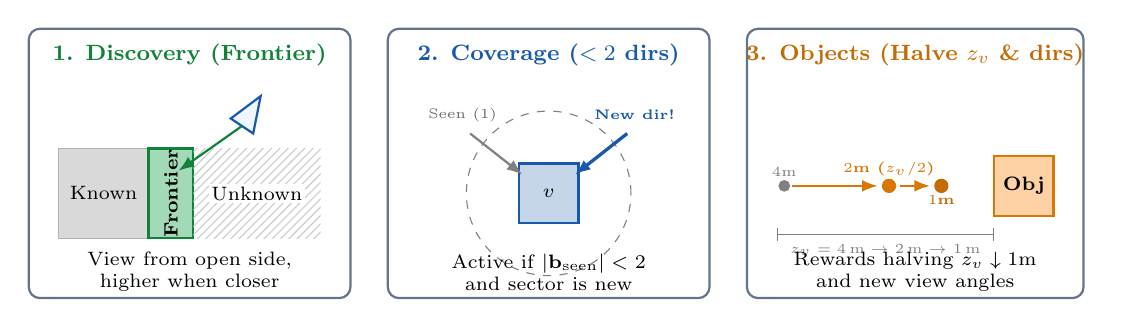
\begin{tikzpicture}[scale=0.95]
    % Panel 1: Discovery
    \begin{scope}[xshift=0cm]
        \draw[thick, rounded corners=4pt, draw=formalborder] (0,0) rectangle (4.3, 3.6);
        \node[font=\footnotesize\bfseries, text=accentgreen!80!black] at (2.15, 3.25) {1. Discovery (Frontier)};
        % Known voxels
        \fill[gray!30, draw=gray!60] (0.4, 0.8) rectangle (1.6, 2.0);
        \node[font=\scriptsize] at (1.0, 1.4) {Known};
        % Frontier voxel
        \fill[accentgreen!40, draw=accentgreen!80!black, thick] (1.6, 0.8) rectangle (2.2, 2.0);
        \node[font=\scriptsize\bfseries, rotate=90] at (1.9, 1.4) {Frontier};
        % Unknown space
        \fill[pattern=north east lines, pattern color=gray!40] (2.2, 0.8) rectangle (3.9, 2.0);
        \node[font=\scriptsize, fill=white, inner sep=1pt] at (3.05, 1.4) {Unknown};
        % Camera looking at open side
        \draw[thick, primaryblue, fill=lightbg] (3.1, 2.7) -- (2.7, 2.4) -- (3.0, 2.2) -- cycle;
        \draw[-{Latex[length=2mm]}, thick, accentgreen!80!black] (2.85, 2.3) -- (2.0, 1.7);
        \node[font=\scriptsize, align=center] at (2.15, 0.35) {View from open side,\\higher when closer};
    \end{scope}

    % Panel 2: Coverage
    \begin{scope}[xshift=4.8cm]
        \draw[thick, rounded corners=4pt, draw=formalborder] (0,0) rectangle (4.3, 3.6);
        \node[font=\footnotesize\bfseries, text=primaryblue] at (2.15, 3.25) {2. Coverage ($<2$ dirs)};
        % Surface voxel
        \fill[primaryblue!25, draw=primaryblue, thick] (1.75, 1.0) rectangle (2.55, 1.8);
        \node[font=\scriptsize\bfseries] at (2.15, 1.4) {$v$};
        % 24 sector arc
        \draw[dashed, gray] (2.15, 1.4) circle (1.1cm);
        % Seen direction 1
        \draw[-{Latex[length=2mm]}, thick, gray] (1.1, 2.2) -- (1.8, 1.65);
        \node[font=\tiny, text=gray!80!black] at (1.0, 2.45) {Seen (1)};
        % New direction 2
        \draw[-{Latex[length=2mm]}, very thick, primaryblue] (3.2, 2.2) -- (2.5, 1.65);
        \node[font=\tiny\bfseries, text=primaryblue] at (3.3, 2.45) {New dir!};
        \node[font=\scriptsize, align=center] at (2.15, 0.35) {Active if $|\mathbf{b}_{\text{seen}}| < 2$\\and sector is new};
    \end{scope}

    % Panel 3: Objects
    \begin{scope}[xshift=9.6cm]
        \draw[thick, rounded corners=4pt, draw=formalborder] (0,0) rectangle (4.5, 3.6);
        \node[font=\footnotesize\bfseries, text=accentorange!90!black] at (2.25, 3.25) {3. Objects (Halve $z_v$ \& dirs)};
        % Object voxel
        \fill[orange!35, draw=accentorange, thick] (3.3, 1.1) rectangle (4.1, 1.9);
        \node[font=\scriptsize\bfseries] at (3.7, 1.5) {Obj};
        % Distance ticks: 4m, 2m, 1m
        \draw[|-|, thin, gray] (0.4, 0.85) -- (3.3, 0.85) node[midway, below, font=\tiny] {$z_v = 4\text{\,m} \to 2\text{\,m} \to 1\text{\,m}$};
        \filldraw[gray] (0.5, 1.5) circle (2pt) node[above, font=\tiny] {$4\text{m}$};
        \filldraw[accentorange] (1.9, 1.5) circle (2.5pt) node[above, font=\tiny\bfseries] {$2\text{m}$ ($z_v/2$)};
        \filldraw[accentorange!90!black] (2.6, 1.5) circle (2.5pt) node[below, font=\tiny\bfseries] {$1\text{m}$};
        \draw[-{Latex[length=2mm]}, thick, accentorange] (0.6, 1.5) -- (1.75, 1.5);
        \draw[-{Latex[length=2mm]}, thick, accentorange] (2.05, 1.5) -- (2.45, 1.5);
        \node[font=\scriptsize, align=center] at (2.25, 0.35) {Rewards halving $z_v \downarrow 1\text{m}$\\and new view angles};
    \end{scope}
\end{tikzpicture}
\caption{Geometric interpretation of the three voxel signals (Slide 19): (1) \textbf{Discovery} scores frontier voxels viewed from their open side; (2) \textbf{Coverage} scores surfaces seen from fewer than 2 directions when viewed from a new sector; (3) \textbf{Objects} scores foreground objects for each halving of viewing distance down to $1\text{\,m}$ and for novel viewing sectors.}
\label{fig:three_signals}
\end{figure}

\intuitionbox{Channel-Modular Planning: Painting Signals onto Gaussians}{
Notice the architectural elegance emphasized at the bottom of Slide 19: \emph{``Each voxel gets a value per signal; each Gaussian takes the value of its voxel. The planner sees channels: a new signal needs no change to it.''} Just as an RGB image has 3 color channels $(R, G, B)$, we can ``paint'' every Gaussian with a 3-channel utility vector $\mathbf{s}_k = (s_{\text{disc}}, s_{\text{cov}}, s_{\text{obj}})$. A single rasterization pass from candidate pose $T$ produces a 3-channel utility image whose pixel sums tell the planner how much discovery, coverage, and object improvement pose $T$ delivers!
}

\subsection{Looking Ahead: Beam Search and Candidate Rendering \emph{(slides 20--21)}}

A myopic (1-step greedy) planner can easily get trapped in a local corner if moving toward a distant object requires passing through a hallway that offers zero immediate reward on the first step. To plan ahead while keeping computation tractable, Slide 20 employs \textbf{Beam Search} over a discrete action graph of candidate camera moves.

\formalbox{
\begin{algorithm_env}[Multi-Step Horizon Beam Search with Signal Rendering]
\textbf{Parameters:} Beam width $W = 5$ sequences, planning horizon $H = 5$ steps ahead, candidate neighbor action set $\mathcal{A}(T)$ (poses one move away in free voxel space).
\begin{enumerate}[leftmargin=*]
    \item \textbf{Initialization ($h=0$):} Start with the singleton beam $\mathcal{B}_0 = \{ (T_t) \}$ containing the current robot pose $T_t$.
    \item \textbf{Iterative Expansion ($h = 1, \dots, H$):}
    \begin{itemize}
        \item Form the candidate set $\mathcal{C}_h = \{ \tau \oplus T_{\text{next}} \mid \tau \in \mathcal{B}_{h-1},\; T_{\text{next}} \in \mathcal{A}(\text{last}(\tau)) \}$.
        \item For each sequence $\tau' = (T_{t+1}, \dots, T_{t+h}) \in \mathcal{C}_h$, render the signal-painted Gaussian map along the sequence, discounting/zeroing out signals already collected by earlier poses in the same sequence $\tau'$ so that viewing the same surface twice in one trajectory is not double-counted:
        \[
        G(\tau') = \sum_{j=1}^{h} \Delta g\bigl(T_{t+j} \mid T_{t+1}, \dots, T_{t+j-1}\bigr).
        \]
        \item \textbf{Pruning:} Sort $\mathcal{C}_h$ by cumulative score $G(\tau')$ and retain only the top $W = 5$ highest-scoring sequences to form $\mathcal{B}_h$.
    \end{itemize}
    \item \textbf{Execution (Receding Horizon):} Select the highest-scoring sequence $\tau^* = \arg\max_{\tau \in \mathcal{B}_H} G(\tau)$, execute its first move $T_{t+1}^*$, capture a new RGB-D frame, update the maps, and repeat.
\end{enumerate}
\end{algorithm_env}
}

\begin{figure}[htbp]
\centering
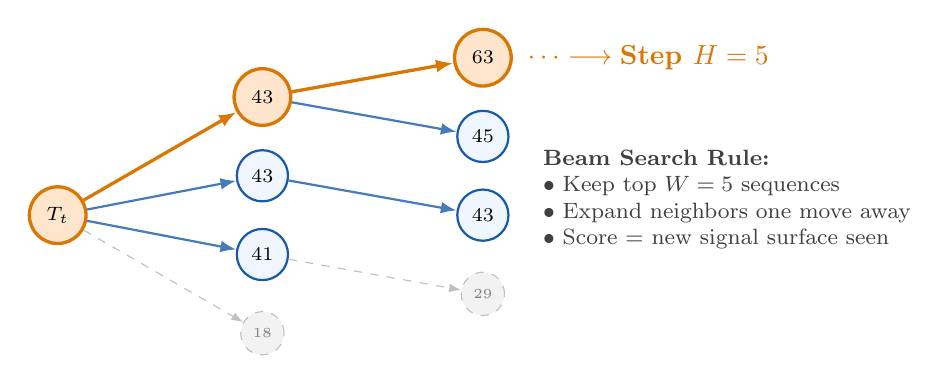
\begin{tikzpicture}[
    level distance=2.3cm,
    node distance=0.8cm,
    cam/.style={circle, draw=primaryblue, thick, fill=lightbg, minimum size=0.65cm, inner sep=1pt, font=\scriptsize\bfseries},
    bestcam/.style={circle, draw=accentorange, very thick, fill=orange!20, minimum size=0.72cm, inner sep=1pt, font=\scriptsize\bfseries},
    pruned/.style={circle, draw=gray!50, dashed, fill=gray!10, minimum size=0.55cm, inner sep=1pt, font=\tiny, text=gray},
    edge/.style={-{Latex[length=2mm]}, thick, draw=primaryblue!80},
    bestedge/.style={-{Latex[length=2.2mm]}, very thick, draw=accentorange},
    prunededge/.style={-{Latex[length=1.5mm]}, dashed, draw=gray!50}
]
    \node[bestcam] (root) at (0,0) {$T_t$};

    % Step 1
    \node[bestcam] (s1_1) at (2.6, 1.5) {$43$};
    \node[cam] (s1_2) at (2.6, 0.5) {$43$};
    \node[cam] (s1_3) at (2.6, -0.5) {$41$};
    \node[pruned] (s1_4) at (2.6, -1.5) {$18$};

    \draw[bestedge] (root) -- (s1_1);
    \draw[edge] (root) -- (s1_2);
    \draw[edge] (root) -- (s1_3);
    \draw[prunededge] (root) -- (s1_4);

    % Step 2
    \node[bestcam] (s2_1) at (5.4, 2.0) {$63$};
    \node[cam] (s2_2) at (5.4, 1.0) {$45$};
    \node[cam] (s2_3) at (5.4, 0.0) {$43$};
    \node[pruned] (s2_4) at (5.4, -1.0) {$29$};

    \draw[bestedge] (s1_1) -- (s2_1);
    \draw[edge] (s1_1) -- (s2_2);
    \draw[edge] (s1_2) -- (s2_3);
    \draw[prunededge] (s1_3) -- (s2_4);

    % Horizon ellipsis
    \node[font=\bfseries, text=accentorange] at (7.5, 2.0) {$\cdots \longrightarrow \text{Step } H=5$};
    \node[font=\footnotesize, align=left, text=darkgray] at (8.5, 0.2) {\textbf{Beam Search Rule:}\\$\bullet$ Keep top $W=5$ sequences\\$\bullet$ Expand neighbors one move away\\$\bullet$ Score $=$ new signal surface seen};
\end{tikzpicture}
\caption{Conceptual illustration of Beam Search over pose sequences (adapted from Slide 20). At each depth, candidate neighbor poses are expanded and scored by rendering the signal-painted Gaussians; only the 5 best sequences (annotated with cumulative scores such as $43 \to 63$) are kept up to horizon $H=5$.}
\label{fig:beam_search}
\end{figure}

\imageplaceholder{Slide 21}{3D room view showing the current camera frustum (black wireframe) and a candidate next pose one move away (red/magenta wireframe) looking toward the coffee table and armchairs, accompanied by the multi-signal renders for Candidate 1.}{Figure: Evaluating candidate poses one move away by rendering the Gaussian map once per signal channel (Slide 21).}

% ============================================================================
\section{Experimental Results and Generalization \emph{(slides 22--25)}}
% ============================================================================

\subsection{A Real Flight: Quantitative Progression and Object Lifecycle \emph{(slides 22--24)}}

Slide 22 presents a full 600-pose autonomous flight in \texttt{room\_0}, tracking both the normalized \textbf{work left} across the three signals (discovery, coverage, objects) and the lifecycle of semantic objects across three states:
\begin{itemize}[leftmargin=*]
    \item \textbf{Found:} Total number of distinct foreground objects discovered in the map so far.
    \item \textbf{Open:} Discovered objects that still require closer views (halving distance down to $1\text{\,m}$) or additional viewing directions.
    \item \textbf{Retired:} Objects whose distance and multi-angle viewing criteria have been completely satisfied ($s_{\text{obj}} = 0$).
\end{itemize}

\begin{figure}[htbp]
\centering
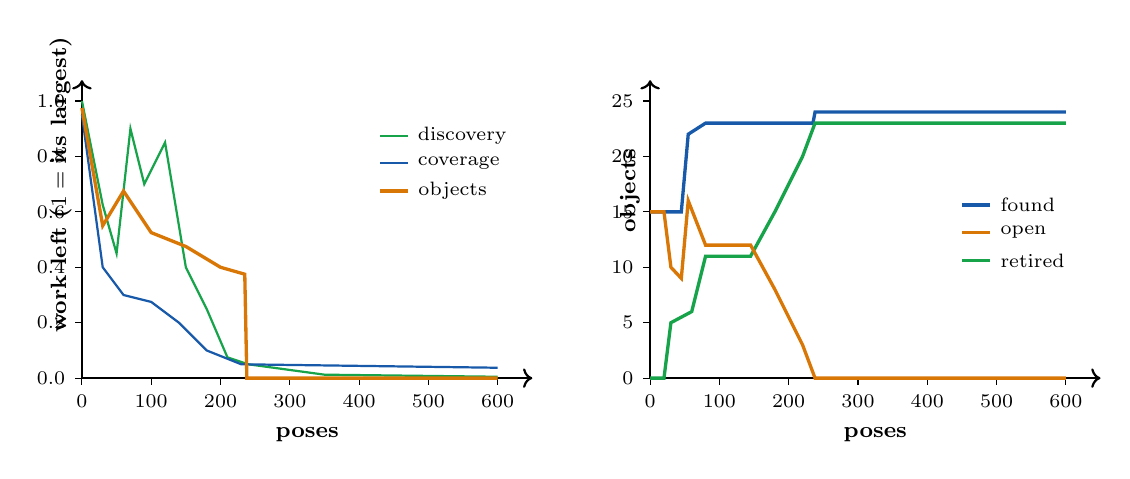
\begin{tikzpicture}[scale=0.88]
    % Left Plot: Work Left vs Poses
    \begin{scope}[xshift=0cm]
        \draw[->, thick] (0,0) -- (6.5,0) node[midway, below=14pt, font=\footnotesize\bfseries] {poses};
        \draw[->, thick] (0,0) -- (0,4.3) node[midway, above=16pt, rotate=90, font=\footnotesize\bfseries] {work left ($1 = \text{its largest}$)};

        % X ticks
        \foreach \x/\lbl in {0/0, 1/100, 2/200, 3/300, 4/400, 5/500, 6/600} {
            \draw (\x, 0) -- (\x, -0.1) node[below, font=\scriptsize] {\lbl};
        }
        % Y ticks
        \foreach \y/\lbl in {0/0.0, 0.8/0.2, 1.6/0.4, 2.4/0.6, 3.2/0.8, 4.0/1.0} {
            \draw (0, \y) -- (-0.1, \y) node[left, font=\scriptsize] {\lbl};
        }

        % Discovery curve (green)
        \draw[thick, accentgreen] (0,4.0) -- (0.3,2.5) -- (0.5,1.8) -- (0.7,3.6) -- (0.9,2.8) -- (1.2,3.4) -- (1.5,1.6) -- (1.8,1.0) -- (2.1,0.3) -- (2.4,0.2) -- (3.5,0.05) -- (6.0,0.02);
        % Coverage curve (blue)
        \draw[thick, primaryblue] (0,3.8) -- (0.3,1.6) -- (0.6,1.2) -- (1.0,1.1) -- (1.4,0.8) -- (1.8,0.4) -- (2.3,0.2) -- (6.0,0.15);
        % Objects curve (orange)
        \draw[very thick, accentorange] (0,3.9) -- (0.3,2.2) -- (0.6,2.7) -- (1.0,2.1) -- (1.5,1.9) -- (2.0,1.6) -- (2.35,1.5) -- (2.38,0.0) -- (6.0,0.0);

        % Legend
        \draw[thick, accentgreen] (4.3, 3.5) -- (4.7, 3.5) node[right, font=\scriptsize, text=black] {discovery};
        \draw[thick, primaryblue] (4.3, 3.1) -- (4.7, 3.1) node[right, font=\scriptsize, text=black] {coverage};
        \draw[very thick, accentorange] (4.3, 2.7) -- (4.7, 2.7) node[right, font=\scriptsize, text=black] {objects};
    \end{scope}

    % Right Plot: Objects Found / Open / Retired vs Poses
    \begin{scope}[xshift=8.2cm]
        \draw[->, thick] (0,0) -- (6.5,0) node[midway, below=14pt, font=\footnotesize\bfseries] {poses};
        \draw[->, thick] (0,0) -- (0,4.3) node[midway, above=14pt, rotate=90, font=\footnotesize\bfseries] {objects};

        % X ticks
        \foreach \x/\lbl in {0/0, 1/100, 2/200, 3/300, 4/400, 5/500, 6/600} {
            \draw (\x, 0) -- (\x, -0.1) node[below, font=\scriptsize] {\lbl};
        }
        % Y ticks (scale: 25 objects -> 4.0 units => 1 obj = 0.16)
        \foreach \y/\lbl in {0/0, 0.8/5, 1.6/10, 2.4/15, 3.2/20, 4.0/25} {
            \draw (0, \y) -- (-0.1, \y) node[left, font=\scriptsize] {\lbl};
        }

        % Found curve (blue)
        \draw[very thick, primaryblue] (0,2.4) -- (0.45,2.4) -- (0.55,3.52) -- (0.8,3.68) -- (2.35,3.68) -- (2.38,3.84) -- (6.0,3.84);
        % Retired curve (green)
        \draw[very thick, accentgreen] (0,0) -- (0.2,0) -- (0.3,0.8) -- (0.6,0.96) -- (0.8,1.76) -- (1.45,1.76) -- (1.8,2.4) -- (2.2,3.2) -- (2.38,3.68) -- (6.0,3.68);
        % Open curve (orange)
        \draw[very thick, accentorange] (0,2.4) -- (0.2,2.4) -- (0.3,1.6) -- (0.45,1.44) -- (0.55,2.56) -- (0.8,1.92) -- (1.45,1.92) -- (1.8,1.28) -- (2.2,0.48) -- (2.38,0.0) -- (6.0,0.0);

        % Legend
        \draw[very thick, primaryblue] (4.5, 2.5) -- (4.9, 2.5) node[right, font=\scriptsize, text=black] {found};
        \draw[very thick, accentorange] (4.5, 2.1) -- (4.9, 2.1) node[right, font=\scriptsize, text=black] {open};
        \draw[very thick, accentgreen] (4.5, 1.7) -- (4.9, 1.7) node[right, font=\scriptsize, text=black] {retired};
    \end{scope}
\end{tikzpicture}
\caption{Quantitative dynamics during a 600-pose autonomous flight in \texttt{room\_0} (redrawn from Slide 22). \textbf{Left:} Normalized work remaining for discovery, coverage, and objects drops sharply and finishes around pose 240. \textbf{Right:} Evolution of \emph{found} (blue, reaching 24 objects), \emph{open} (orange), and \emph{retired} (green) objects; by pose 240, every discovered object has been thoroughly inspected and retired (\texttt{open} $= 0$).}
\label{fig:real_flight_plots}
\end{figure}

\intuitionbox{Reading the Flight Curves on Slide 22}{
Look closely at the two plots in Figure~\ref{fig:real_flight_plots} around poses $50\text{--}120$ and pose $240$:
\begin{enumerate}[leftmargin=*]
    \item \textbf{Temporary spikes in ``work left'':} Around pose 55, the discovery and object curves jump \emph{upward}. Why? Because the robot turns a corner and sees a new part of the room! New frontier voxels appear and the number of \textbf{found} objects jumps from 15 to 23, temporarily increasing the number of \textbf{open} objects waiting for close-up inspection.
    \item \textbf{Task completion around pose 240:} By pose 240, the \textbf{retired} curve (green) catches up to the \textbf{found} curve (blue), driving \textbf{open} objects (orange) and ``work left'' to zero. This directly motivates one of the open research questions on Slide 26: \emph{knowing automatically when to stop!}
\end{enumerate}
}

\imageplaceholder{Slide 22 (top) and Slides 23--24}{Top of Slide 22: 3D trajectory (blue path) overlaid on RGB and semantic maps at pose 600 of 600. Slide 23: Full-bleed photorealistic online Gaussian render of room\_0. Slide 24: 2x2 grid of online mapped scenes: room\_2, office\_0, office\_2, office\_3.}{Figure: Online 3D Gaussian reconstructions and trajectories across Replica dataset rooms (\texttt{room\_0}, \texttt{room\_2}, \texttt{office\_0}, \texttt{office\_2}, \texttt{office\_3}) from Slides 22--24.}

\subsection{Same System, Another Task: Object Navigation \emph{(slide 25)}}

A major strength of separating the \textbf{Planner/Renderer} from the \textbf{Signal Channels} is that changing the robot's task requires \textbf{zero changes} to the Gaussian map, differentiable renderer, or beam search planner—only the signals painted onto the Gaussians change. Slide 25 demonstrates this by contrasting \textbf{Object Mapping} with \textbf{Object Navigation} (\emph{``Find a chair in a house never seen before''}):

\begin{itemize}[leftmargin=*]
    \item \textbf{Frontier Signal:} Rewards visible frontiers in line of sight to explore unknown rooms.
    \item \textbf{Relay Signal:} Guides the robot toward frontiers that are currently \emph{out of sight} (e.g., through a doorway or corridor connecting rooms).
    \item \textbf{Target Signal:} A Vision-Language Model (VLM) detects bounding boxes of the target category (e.g., ``chair'') in each RGB frame; Gaussians falling inside the detected 2D boxes receive high target signal values.
    \item \textbf{Stopping Condition:} The robot stops automatically once it maneuvers close to a confirmed target object.
\end{itemize}

% ============================================================================
\section{Summary and Key Takeaways \emph{(slide 26)}}
% ============================================================================

\subsection{Comparison of Paradigms and Task Configurations}

Table~\ref{tab:comparison} synthesizes the active perception methods and task configurations covered across the lecture.

\begin{table}[htbp]
\centering
\small
\renewcommand{\arraystretch}{1.35}
\begin{tabular}{p{3.0cm} p{3.4cm} p{3.6cm} p{4.0cm}}
\toprule
\textbf{Method / Task} & \textbf{Scene Representation} & \textbf{Signals Painted on Gaussians} & \textbf{Key Properties \& Limitations} \\
\midrule
\textbf{Passive 3DGS} \newline \emph{(Kerbl et al., 2023)} & $M$ anisotropic 3D Gaussians $(\boldsymbol{\mu}_k, \boldsymbol{\Sigma}_k, \alpha_k, \mathbf{c}_k)$ & RGB color $\mathbf{c}_k$ (for photometric loss $\mathcal{L}$) & Fast rendering; no viewpoint planning; suffers under limited view budgets. \\
\addlinespace[3pt]
\textbf{MAGICIAN} \newline \emph{(Li et al., CVPR 2026)} & Reconstructed Point Cloud $+$ Volume Occupancy Net $\to$ \textbf{Imagined Gaussians} & Opacity $= \hat{p}_{\text{occ}}$, \newline Color $=$ Novelty $\in \{0,1\}$ & Beam search over trajectories; maximizes raw surface coverage; ignores semantics \& viewing distance ($1$ glance $= 0$ novelty). \\
\addlinespace[3pt]
\textbf{Semantic Object Mapping} \newline \emph{(This Lecture, Slides 12--24)} & Coupled \textbf{Online Gaussian Map} (4-slot voting) $+$ \textbf{5\,cm Voxel State} & 1. \textbf{Discovery} (frontiers) \newline 2. \textbf{Coverage} ($<2$ dirs) \newline 3. \textbf{Objects} (halve $z_v \downarrow 1\text{m}$, new dirs) & Depth-gated semantic voting; floater removal; maps every foreground object closely from multiple angles. \\
\addlinespace[3pt]
\textbf{Object Navigation} \newline \emph{(This Lecture, Slide 25)} & Same Online Gaussian Map $+$ Voxel Planning State & 1. \textbf{Frontier} (in sight) \newline 2. \textbf{Relay} (out-of-sight door) \newline 3. \textbf{Target} (VLM 2D boxes) & Same renderer and 5-step beam search; stops when close to a confirmed target. \\
\bottomrule
\end{tabular}
\caption{Comparison of passive 3DGS, coverage-driven MAGICIAN, Semantic Object Mapping, and Object Navigation.}
\label{tab:comparison}
\end{table}

\begin{figure}[htbp]
\centering
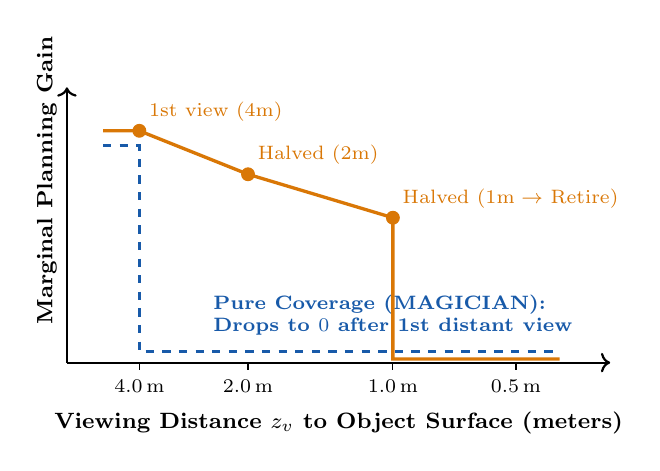
\begin{tikzpicture}[scale=0.92]
    \draw[->, thick] (0,0) -- (7.5,0) node[midway, below=14pt, font=\footnotesize\bfseries] {Viewing Distance $z_v$ to Object Surface (meters)};
    \draw[->, thick] (0,0) -- (0,3.8) node[midway, above=16pt, rotate=90, font=\footnotesize\bfseries] {Marginal Planning Gain};

    % X ticks (distances from 4m down to 0.5m)
    \foreach \x/\lbl in {1/4.0\,\text{m}, 2.5/2.0\,\text{m}, 4.5/1.0\,\text{m}, 6.2/0.5\,\text{m}} {
        \draw (\x, 0) -- (\x, -0.1) node[below, font=\scriptsize] {\lbl};
    }

    % MAGICIAN curve (flat zero after first seen at 4m)
    \draw[very thick, dashed, primaryblue] (0.5, 3.0) -- (1.0, 3.0) -- (1.0, 0.15) -- (6.8, 0.15);
    \node[font=\scriptsize\bfseries, text=primaryblue, align=left] at (4.5, 0.65) {Pure Coverage (MAGICIAN):\\Drops to $0$ after 1st distant view};

    % Object-Centric Step/Halving Reward curve
    \draw[very thick, accentorange] (0.5, 3.2) -- (1.0, 3.2) -- (2.5, 2.6) -- (4.5, 2.0) -- (4.5, 0.05) -- (6.8, 0.05);
    \filldraw[accentorange] (1.0, 3.2) circle (2.5pt) node[above right, font=\scriptsize] {1st view ($4\text{m}$)};
    \filldraw[accentorange] (2.5, 2.6) circle (2.5pt) node[above right, font=\scriptsize] {Halved ($2\text{m}$)};
    \filldraw[accentorange] (4.5, 2.0) circle (2.5pt) node[above right, font=\scriptsize] {Halved ($1\text{m} \to$ Retire)};
\end{tikzpicture}
\caption{Qualitative comparison of marginal information gain as a function of viewing distance $z_v$ after an object is first spotted at $4.0\text{\,m}$. Pure coverage planners drop to zero gain immediately after the first distant observation, whereas the Object signal continues rewarding closer views (each distance halving down to $1.0\text{\,m}$) until the object is retired.}
\label{fig:qualitative_comparison}
\end{figure}

\subsection{Key Takeaways and Open Directions \emph{(slide 26)}}

\begin{itemize}[leftmargin=*]
    \item \textbf{1. Render anything:} By replacing each Gaussian's RGB color $\mathbf{c}_k$ with a task utility signal $s_k$, candidate viewpoints are scored in a single fast, occlusion-aware rasterization pass: $g(T, \tau) = \sum_u \sum_k w_k(u) s_k$.
    \item \textbf{2. Plan on what you build:} The Online Gaussian Map and the $5\text{\,cm}$ Voxel Planning State share information bidirectionally at every frame—Gaussians vote on depth-gated pixel semantics and label the voxels, while depth-raycasted voxels remove mid-air Gaussian floaters and compute spatial signals.
    \item \textbf{3. Value is a design choice:} Discovering unknown frontiers, covering single-sided surfaces, and getting closer to semantic objects (or navigating to a VLM-detected chair) are simply different signal channels fed into the exact same renderer and horizon-5 beam search planner.
    \item \textbf{4. Open problems \& project ideas:} Key open challenges include learning \textbf{when to stop} automatically once scene work is exhausted, handling \textbf{dynamic/moving scenes}, operating under \textbf{unknown/noisy camera poses} (Active SLAM), deploying on a \textbf{real flying robot}, and designing new signal channels such as open-vocabulary \textbf{text queries}.
\end{itemize}

\vspace{8pt}
\noindent\textbf{Primary References Cited in the Lecture:}
\begin{enumerate}[leftmargin=*, label={[\arabic*]}]
    \item Kerbl, B., Kopanas, G., Leimk{\"u}hler, T., \& Drettakis, G. (2023). \emph{3D Gaussian splatting for real-time radiance field rendering.} ACM Transactions on Graphics (TOG), 42(4), 1--14.
    \item Li, S., et al. (2026). \emph{MAGICIAN: Efficient long-term planning with imagined Gaussians for active mapping.} In Proceedings of the IEEE/CVF Conference on Computer Vision and Pattern Recognition (CVPR 2026).
\end{enumerate}

\end{document}
